\documentclass[12pt,letterpaper]{article}
\usepackage{graphicx,textcomp}
\usepackage{natbib}
\usepackage{setspace}
\usepackage{fullpage}
\usepackage{color}
\usepackage[reqno]{amsmath}
\usepackage{amsthm}
\usepackage{fancyvrb}
\usepackage{amssymb,enumerate}
\usepackage[all]{xy}
\usepackage{endnotes}
\usepackage{lscape}
\newtheorem{com}{Comment}
\usepackage{float}
\usepackage{hyperref}
\newtheorem{lem} {Lemma}
\newtheorem{prop}{Proposition}
\newtheorem{thm}{Theorem}
\newtheorem{defn}{Definition}
\newtheorem{cor}{Corollary}
\newtheorem{obs}{Observation}
\usepackage[compact]{titlesec}
\usepackage{dcolumn}
\usepackage{tikz}
\usetikzlibrary{arrows}
\usepackage{multirow}
\usepackage{xcolor}
\newcolumntype{.}{D{.}{.}{-1}}
\newcolumntype{d}[1]{D{.}{.}{#1}}
\definecolor{light-gray}{gray}{0.65}
\usepackage{url}
\usepackage{listings}
\usepackage{color}

\definecolor{codegreen}{rgb}{0,0.6,0}
\definecolor{codegray}{rgb}{0.5,0.5,0.5}
\definecolor{codepurple}{rgb}{0.58,0,0.82}
\definecolor{backcolour}{rgb}{0.95,0.95,0.92}

\lstdefinestyle{mystyle}{
	backgroundcolor=\color{backcolour},   
	commentstyle=\color{codegreen},
	keywordstyle=\color{magenta},
	numberstyle=\tiny\color{codegray},
	stringstyle=\color{codepurple},
	basicstyle=\footnotesize,
	breakatwhitespace=false,         
	breaklines=true,                 
	captionpos=b,                    
	keepspaces=true,                 
	numbers=left,                    
	numbersep=5pt,                  
	showspaces=false,                
	showstringspaces=false,
	showtabs=false,                  
	tabsize=2
}
\lstset{style=mystyle}
\newcommand{\Sref}[1]{Section~\ref{#1}}
\newtheorem{hyp}{Hypothesis}

\title{Problem Set 6}
\date{Due: May 1, 2020}
\author{QTM 200: Applied Regression Analysis}

\begin{document}
	\maketitle
	
	\section*{Instructions}
	\begin{itemize}
		\item Please show your work! You may lose points by simply writing in the answer. If the problem requires you to execute commands in \texttt{R}, please include the code you used to get your answers. Please also include the \texttt{.R} file that contains your code. If you are not sure if work needs to be shown for a particular problem, please ask.
		\item Your homework should be submitted electronically on the course GitHub page in \texttt{.pdf} form.
		\item This problem set is due before midnight on Friday, May 1, 2020. No late assignments will be accepted.
		\item Total available points for this homework is 100.
	\end{itemize}
	
	\vspace{.5cm}
\section*{Question 1 (50 points): Biology}
\vspace{.25cm}
\noindent Load in the data labelled \texttt{cholesterol.csv} on GitHub, which contains an observational study of 315 observations.

\begin{itemize}
	\item
	Response variable: 
	\begin{itemize}
		\item \texttt{cholCat}: 1 if the individual has high cholesterol; 0 if the individual does not have high cholesterol
	\end{itemize}
	\item
	Explanatory variables: 
	\begin{itemize}
		\item
		\texttt{sex}: 1 Male; 0 Female
		\item
		\texttt{fat}: grams of fat consumed per day
		
	\end{itemize}
	
\end{itemize}

\newpage
\noindent Please answer the following questions:

\begin{enumerate}
	\item
	We are interested in predicting the cholesterol category based on sex and fat intake.
	\begin{enumerate}
		\item
		Fit an additive model. Provide the summary output, the global null hypothesis, and $p$-value. Please describe the results and provide a conclusion. 
		
		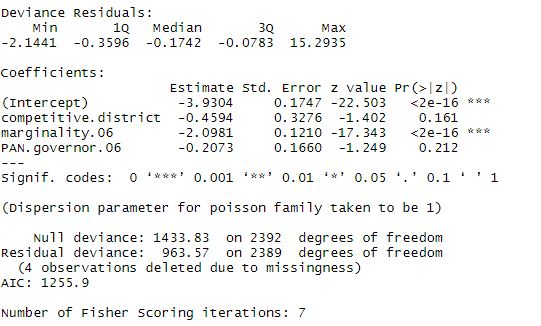
\includegraphics[scale=.75]{summary table 1.jpg}
		
		\lstinputlisting[language=R, firstline=49, lastline=54]{PS06_answers.R}
		
		%\item
		%How many iterations did it take to find the maximum likelihood estimates?
	\end{enumerate}
	
	\item
	If explanatory variables are significant in this model, then
	\begin{enumerate}
		\item
		For women, how does increasing their fat intake by 1 gram per day change their odds on being in the high cholesterol group? (Interpretation of a coefficient) 
		
		\lstinputlisting[language=R, firstline=59, lastline=59]{PS06_answers.R}
		
		\item
		For men, how does increasing their fat intake by 1 gram per day change their odds on being in the high cholesterol group? (Interpretation of a coefficient) 
		
			\lstinputlisting[language=R, firstline=63, lastline=63]{PS06_answers.R}
		
		\item
		What is the estimated probability of a woman with a fat intake of 100 grams per day being in the high cholesterol group?
		
			\lstinputlisting[language=R, firstline=67, lastline=67]{PS06_answers.R}
		 
		\item
		Would the answers to 2a and 2b potentially change if we included the interaction term in this model? Why? 
		\begin{itemize}
			\item Perform a test to see if including an interaction is appropriate.
		\end{itemize} 
		
		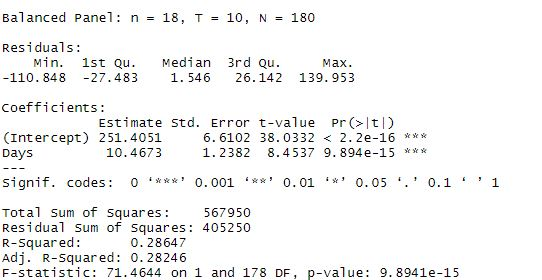
\includegraphics[scale=.75]{summary table 2.jpg}
		
			\lstinputlisting[language=R, firstline=70, lastline=72]{PS06_answers.R}
		
%		\item
%		If you consider all people who have a given fat intake, how does changing from being a female to a male change the odds on being in the high cholesterol group? (For additive model)
	
		
	\end{enumerate}
\end{enumerate}
\newpage


\section*{Question 2 (50 points): Political Economy}
\vspace{.25cm}
\noindent We are interested in how governments' management of public resources impacts economic prosperity. Our data come from \href{https://www.researchgate.net/profile/Adam_Przeworski/publication/240357392_Classifying_Political_Regimes/links/0deec532194849aefa000000/Classifying-Political-Regimes.pdf}{Alvarez, Cheibub, Limongi, and Przeworski (1996)} and is labelled \texttt{gdpChange.csv} on GitHub. The dataset covers 135 countries observed between 1950 or the year of independence or the first year forwhich data on economic growth are available ("entry year"), and 1990 or the last year for which data on economic growth are available ("exit year"). The unit of analysis is a particular country during a particular year, for a total $>$ 3,500 observations. 

\begin{itemize}
	\item
	Response variable: 
	\begin{itemize}
		\item \texttt{GDPWdiff}: Difference in GDP between year $t$ and $t-1$. Possible categories include: "positive", "negative", or "no change"
	\end{itemize}
	\item
	Explanatory variables: 
	\begin{itemize}
		\item
		\texttt{REG}: 1=Democracy; 0=Non-Democracy
		\item
		\texttt{OIL}: 1=if the average ratio of fuel exports to total exports in 1984-86exceeded 50\%; 0= otherwise
		\item \texttt{EDT}: Cumulative years of education of the average member of the labor force
	\end{itemize}
	
\end{itemize}

\noindent Please answer the following questions:

\begin{enumerate}
	\item Construct and interpret an unordered multinomial logit with \texttt{GDPWdiff} as the output and "no change" as the reference category, including the estimated cutoff points and coefficients. 
	
	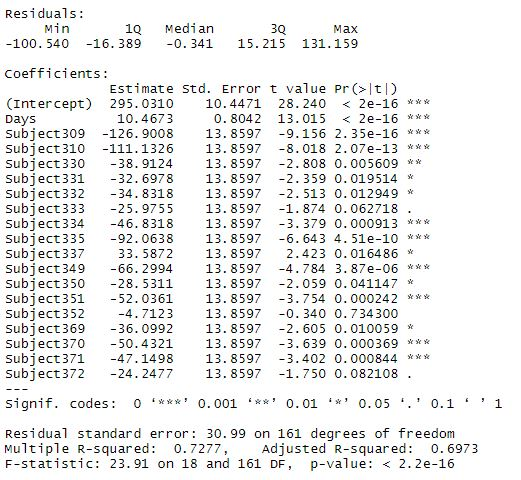
\includegraphics[scale=.75]{summary table 3.jpg}
	
	\lstinputlisting[language=R, firstline=81, lastline=88]{PS06_answers.R}
	
	\item Construct and interpret an ordered multinomial logit with \texttt{GDPWdiff} as the outcome variable, including the estimated cutoff points and coefficients.
	
	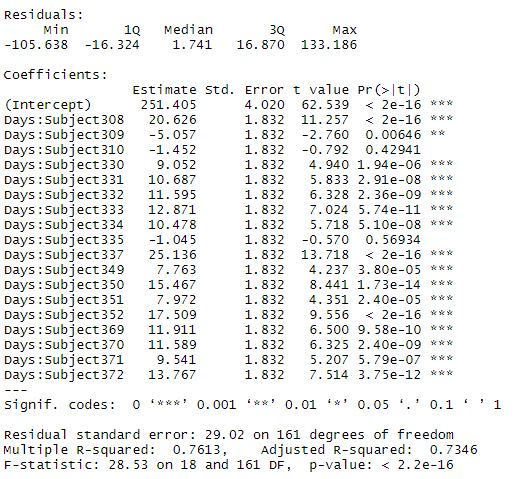
\includegraphics[scale=.75]{summary table 4.jpg}
	
	\lstinputlisting[language=R, firstline=91, lastline=93]{PS06_answers.R}
	
\end{enumerate}


\end{document}
